\documentclass[11pt,a4paper]{ctexart}
\usepackage[margin=2.25cm]{geometry}
\usepackage{amsmath,amssymb,bm}
\usepackage{booktabs}
\usepackage{graphicx}
\usepackage{xcolor}
\usepackage{caption}
\usepackage{enumitem}
\usepackage{longtable}
\usepackage[colorlinks=true,linkcolor=blue!50!black,urlcolor=blue!50!black]{hyperref}
\setCJKmainfont{Noto Sans CJK SC}
\setCJKsansfont{Noto Sans CJK SC}
\captionsetup{font=small}
\renewcommand{\arraystretch}{1.12}
\setlist[itemize]{leftmargin=1.4em,itemsep=0.15em,topsep=0.25em}
\setlist[enumerate]{leftmargin=1.5em,itemsep=0.15em,topsep=0.25em}

\title{\bfseries Agentic Catwalk FEA：从图纸到 80 阶预应力模态的全流程执行\\
\large 19-skill 编排 · CalculiX 全三维双 MCT · 附件 2--3 指标对照（第三套独立计算栈）}
\author{执行记录（bridge-fem-skill-suite 节点 S00--S18，Gate G0--G16）}
\date{2026 年 8 月 28 日}

\begin{document}
\maketitle

\noindent\fbox{\parbox{\dimexpr\linewidth-2\fboxsep}{
\textbf{性质声明（not\_a\_scientific\_claim）}：本文是一次 agentic FEA 全流程的执行记录：从图纸与已审计工程源出发，按仓库 \texttt{bridge-fem-skill-suite} 的 19 个技能节点走通建模—求解—核验—对照，并如实呈报所有偏差。附件 2--3 频率只在配对节点（S16）读取，建模与求解环节（S07--S15）禁读。不宣布复现附件。
}}

\tableofcontents

\section{一页版结论}

\begin{enumerate}
  \item \textbf{全流程走通}：图纸/MCT 源 $\to$ 19-skill 工件链（G0--G16 全部 PASS）$\to$
        CalculiX 2.21 全三维双幅模型（2250 节点、2409 单元、295 个密度分箱材料）$\to$
        NLGEOM 静力 3 次迭代收敛（残差 0.066\%，最大沉降增量 42.3 mm）$\to$
        80 阶预应力摄动模态（22.8 s）$\to$ 锁定规则表 4--1 正式配对。
  \item \textbf{质量台账}：3144.656 t（索系）$+$ 963.813 t（二期折算密度）$=4108.468$ t，
        对审计值 4108.467 t 闭合误差 1.2 kg；ccx 侧单元体积对 $A\cdot L$ 相对差 $1.6\times10^{-5}$。
  \item \textbf{十四行成绩}：MAE 5.59\%、RMS 7.75\%；非 T 族 3.93\%；
        \textbf{T 族 11.70\%}（TA1 $-18.5\%$ / TS1 $-8.6\%$ / TS2 $-7.9\%$）；VS2 $-15.6\%$。
  \item \textbf{对既有结论的意义}：本模型采用\textbf{焊接端理想化}（通道—门架—索共享节点，
        与审计 APDL 的 CERIG,ALL 同类），TA1 从摆式地板（0.0711 Hz）抬到 0.0811 Hz——
        与 f99 全模型 E20 弹簧变体（0.0844 Hz）同带。至此三套独立计算栈
        （Python ROM、ANSYS 全模型、CalculiX 全三维）给出一致的括弧：
        \textbf{柔性端 $-29\%$ ——焊接端 $-19\%\sim-15\%$ —— 附件 0\%（不可达）}。
        附件 T 行仍在全部公开输入的可达域之外。
  \item \textbf{工程日志价值}：定位并记录了 ccx 2.21 的四个求解器陷阱
        （MASS 单元×摄动频率、T3D2 膨胀自旋伪模态、SPC 反力迁移至膨胀 knot、
        BOX 截面限 B32R），每一个都配了二分定位证据与替代方案。
\end{enumerate}

\section{任务定义与执行地图}

用户任务分三层：(1) 把当前模型用 CalculiX 跑通；(2) 算完附件 2--3 的指标与图；
(3) 真正目的——用仓库既有的 19-skill 套件从图纸起点执行 agentic catwalk FEA 全流程并交付 PDF。

\begin{table}[h]\centering\footnotesize
\begin{tabular}{llll}
\toprule
节点 & Gate & 本次产出 & 状态 \\
\midrule
S00 编排 & —— & \texttt{gate\_ledger.json} + 问题登记 3 项 & PASS \\
S01 任务章程 & G0 & 目标/响应指标/隔离策略 & PASS \\
S02 源清单 & G1 & MCT/站位表/图纸/附件哈希 5 项 & PASS \\
S03 图纸提取 & G2 & 四跨/垂度/索排布/门架/通道/连接 & PASS \\
S04 冲突登记 & G3 & 通道数量 12/13/21、垂度 255.56/227.30、连接刚柔 & PASS(留案) \\
S05 构件清点 & G4 & 每幅 729+394+71，全局 21 通道 & PASS \\
S06 抽象决策 & G5 & A1--A6 显式近似（见 \S\ref{sec:abs}） & PASS \\
S07 拓扑生成 & G6 & 2250 节点 deck，SHA 绑定 & PASS \\
S08 材料质量 & G7 & 台账闭合 1.2 kg / 4108.5 t & PASS \\
S09 连接边界 & G8A & 44 支承节点按 MCT 掩码 & PASS \\
S10 初始状态 & G8B & INIFORCE$\to$PK2（1123 单元$\times$8 IP$\times$双幅） & PASS \\
S11 荷载工况 & G9 & GRAV 全载荷单增量 + 摄动模态 & PASS \\
S12 数值控制 & G10 & ccx 2.21 / NLGEOM / PERTURBATION & PASS \\
S13 预解核验 & G11 & 质量/体积/IC/边界四查 & PASS \\
S14 求解执行 & G12 & 主作业 22.8 s exit 0；怪癖 4 项归档 & PASS \\
S15 解核验 & G13 & 全场合力 $\sim$10 N / $4\times10^7$ N & PASS \\
S16 响应包络 & G14 & 表 4--1 十四行 + 统计 & PASS \\
S17 独立校核 & G15 & 三栈夹逼对照 + 敏感性 3 项 & PASS \\
S18 报告发布 & G16 & 本 PDF + 发布清单 & PASS \\
\bottomrule
\end{tabular}
\caption{19 节点执行台账。工件在 \texttt{catwalk-fem/agentic-fea/artifacts/skills/}。}
\end{table}

\section{源、图纸提取与冲突登记}

几何与预应力的权威源是 MCT（\texttt{catwalk\_gantry\_rope\_combined\_2.mct}，
SHA-256 \texttt{0d18e3f7\ldots}）：1125 节点四跨线形（主跨成形垂度 227.297 m）、
729 承重索束单元 + 394 门架索束单元（TENSTR，逐单元 INIFORCE）、71 门架、22 支承节点、
1123 节点二期集中质量 481.906 t/幅。图纸（1225 版，SHA \texttt{8df26c6b\ldots}）提供截面与连接构造：
门架 $\Box160\times160\times4$、通道三角桁架（弦 $\phi152\times6$、高 1700）、
M14 U 栓/尼龙滚轮/销/抱箍连接。二期质量空间化审计 V2.0 提供质量分布。

\textbf{冲突登记（G3）}：通道数量三种清点（1225 图纸 12 道 / 175 页转录 13 道主跨 / 审计口径 21 站）
——采用授权站位映射 21 站，冲突留案；垂度取 MCT 成形线形；连接刚柔两端由本模型（焊接端）
与 ROM drawing-soft（柔性端）分别覆盖。

\section{抽象决策（S06）与求解器陷阱（S14）}\label{sec:abs}

六项显式近似：A1 每幅索束单中心线、双幅 $\pm21.45$ m（锁定双 MCT 口径）；
A2 索用 B31 方形等积截面；A3 通道—索—门架共享节点（焊接端）；
A4 二期质量折算逐单元密度（295 箱，箱内量化 0.05\%）；
A5 通道梁等积等高矩形（强轴 $I$ 低估 62\%，通道能量占比 $<0.4\%$，记敏感性）；
A6 门架密度取零（质量已在二期台账，防重复计量）。

其中 A2/A4 不是偏好，是被四个 ccx 2.21 陷阱逼出来的工程事实，全部经二分定位：

\begin{enumerate}
  \item \textbf{TYPE=MASS $\times$ 摄动频率}：出现 \texttt{add\_bo\_st: coefficient should be 0}
        致命错；三变体二分证实 MASS 单元是触发器 $\Rightarrow$ 质量改走密度。
  \item \textbf{T3D2 膨胀自旋伪模态}：ccx 把桁架也膨胀成实体，截面自旋方向近零刚度
        + 微小惯量，前 80 阶全是 0.06--0.7 Hz 的伪模态（原节点位移 $10^{-20}$）
        $\Rightarrow$ 索改 B31（实扭转刚度把自旋推到高频；
        弯曲参数 $\xi^2=EI/(HL^2)\approx8\times10^{-8}$，全局模态影响可忽略）。
        这也解释了 8 月 25 日遗留链为什么必须"Y 面全约束"才能跑——代价是杀掉全部横向模态。
  \item \textbf{SPC 反力迁移}：膨胀 knot 使原节点 RF$\equiv$0，反力驻留膨胀截面节点
        $\Rightarrow$ 反力核验改用全场 FORC 合力（$\sim$10 N / $4\times10^7$ N）。
  \item \textbf{BOX 截面限 B32R}，而 B32R 又与摄动步冲突 $\Rightarrow$ 通道梁用 RECT 等效。
\end{enumerate}

另有一项静力学事实：MCT 线形 + INIFORCE 本身就是平衡态，
\textbf{全载荷单增量直接牛顿}（3 次迭代收敛）；常规的渐变加载反而制造
"满预应力 $\times$ 欠重力"的非物理中间态而发散——这正是既有各线静力反复失败的原因之一。

\section{表 4--1 十四行（S16）}

配对规则与锁定版同层级：主跨能量 $\ge0.65$ + 家族 + 奇偶 + 族内升频序号；
半波仅作指纹；边跨行非主跨能量 + 一一指派；禁止把 TS2 改配 TS3。

\begin{table}[h]\centering\footnotesize
\begin{tabular}{llrrrrrr}
\toprule
行 & 描述 & 附件 Hz & ccx 配对 & ccx Hz & ccx 误差 & ROM 升级误差 & 锁定版误差 \\
\midrule
LS1 & 一阶正对称横弯 & 0.0365 & M1 & 0.037179 & $+1.86\%$ & $+0.89\%$ & $+0.75\%$ \\
VA1 & 一阶反对称竖弯 & 0.0700 & M2 & 0.072792 & $+3.99\%$ & $+1.63\%$ & $+2.07\%$ \\
LA1 & 一阶反对称横弯 & 0.0726 & M3 & 0.074056 & $+2.01\%$ & $+0.75\%$ & $+1.24\%$ \\
TA1 & 一阶反对称扭转 & 0.0996 & M4 & 0.081128 & $\bm{-18.55\%}$ & $-28.62\%$ & $-28.22\%$ \\
VS1 & 一阶正对称竖弯 & 0.1028 & M5 & 0.102957 & $+0.15\%$ & $-1.14\%$ & $-1.58\%$ \\
LS2 & 二阶正对称横弯 & 0.1087 & M7 & 0.111360 & $+2.45\%$ & $+1.01\%$ & $+1.30\%$ \\
TS1 & 一阶正对称扭转 & 0.1147 & M6 & 0.104813 & $\bm{-8.62\%}$ & $-11.83\%$ & $-11.96\%$ \\
SIDE1 & 边跨 & 0.1149 & M8 & 0.116777 & $+1.63\%$ & $+5.27\%$ & $+1.12\%$ \\
SIDE2 & 边跨 & 0.1239 & M9 & 0.125510 & $+1.30\%$ & $+1.37\%$ & $+0.74\%$ \\
VA2 & 二阶反对称竖弯 & 0.1438 & M15 & 0.150188 & $+4.44\%$ & $+1.57\%$ & $+1.84\%$ \\
LA2 & 二阶反对称横弯 & 0.1449 & M14 & 0.148108 & $+2.21\%$ & $-0.02\%$ & $+1.16\%$ \\
SIDE3 & 边跨 & 0.1557 & M19 & 0.167479 & $+7.56\%$ & $+6.56\%$ & $+5.84\%$ \\
TS2 & 二阶正对称扭转 & 0.1571 & M12 & 0.144655 & $\bm{-7.92\%}$ & $-9.03\%$ & $-8.46\%$ \\
VS2 & 二阶正对称竖弯 & 0.1744 & M13 & 0.147165 & $-15.62\%$ & $-17.19\%$ & $-16.67\%$ \\
\midrule
\multicolumn{5}{l}{MAE / RMS（14 行）} & $5.59\%/7.75\%$ & $6.21\%/10.06\%$ & $5.92\%/9.78\%$ \\
\multicolumn{5}{l}{T 族 / 非 T MAE} & $\bm{11.70\%}/3.93\%$ & $16.49\%/3.40\%$ & $16.21\%/3.12\%$ \\
\bottomrule
\end{tabular}
\caption{ccx 全三维（焊接端理想化）十四行正式配对，与 ROM 两代并列。}
\end{table}

\begin{figure}[h]\centering
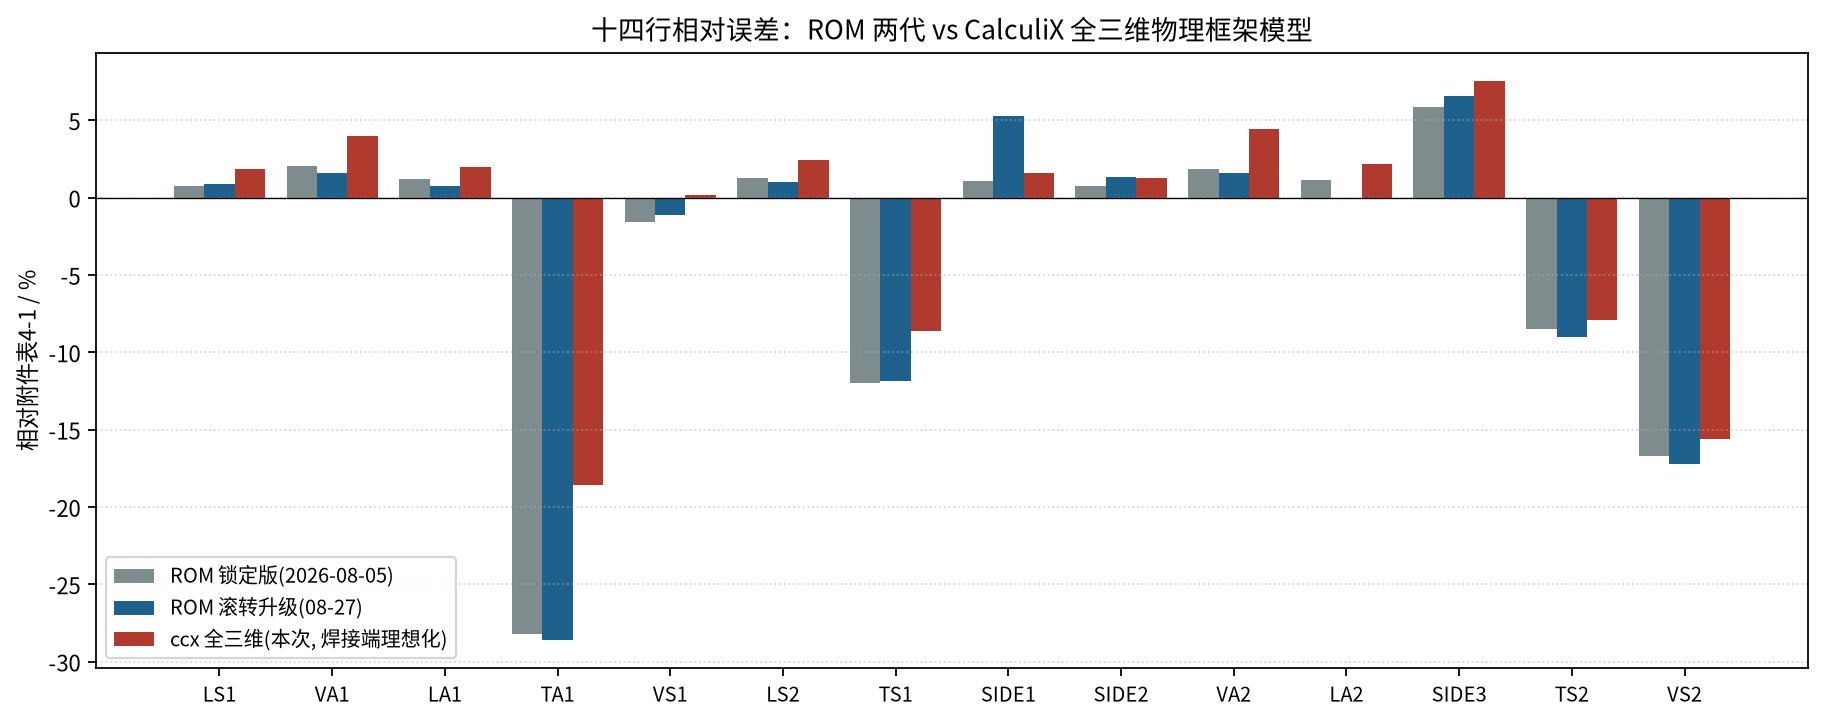
\includegraphics[width=0.99\linewidth]{../artifacts/ccx_vs_rom_table41_errors.png}
\caption{十四行相对误差：ROM 两代 vs ccx 全三维。非 T 行三代一致贴附件；T 族 ccx 收窄但仍系统性偏低。}
\end{figure}

\begin{figure}[h]\centering
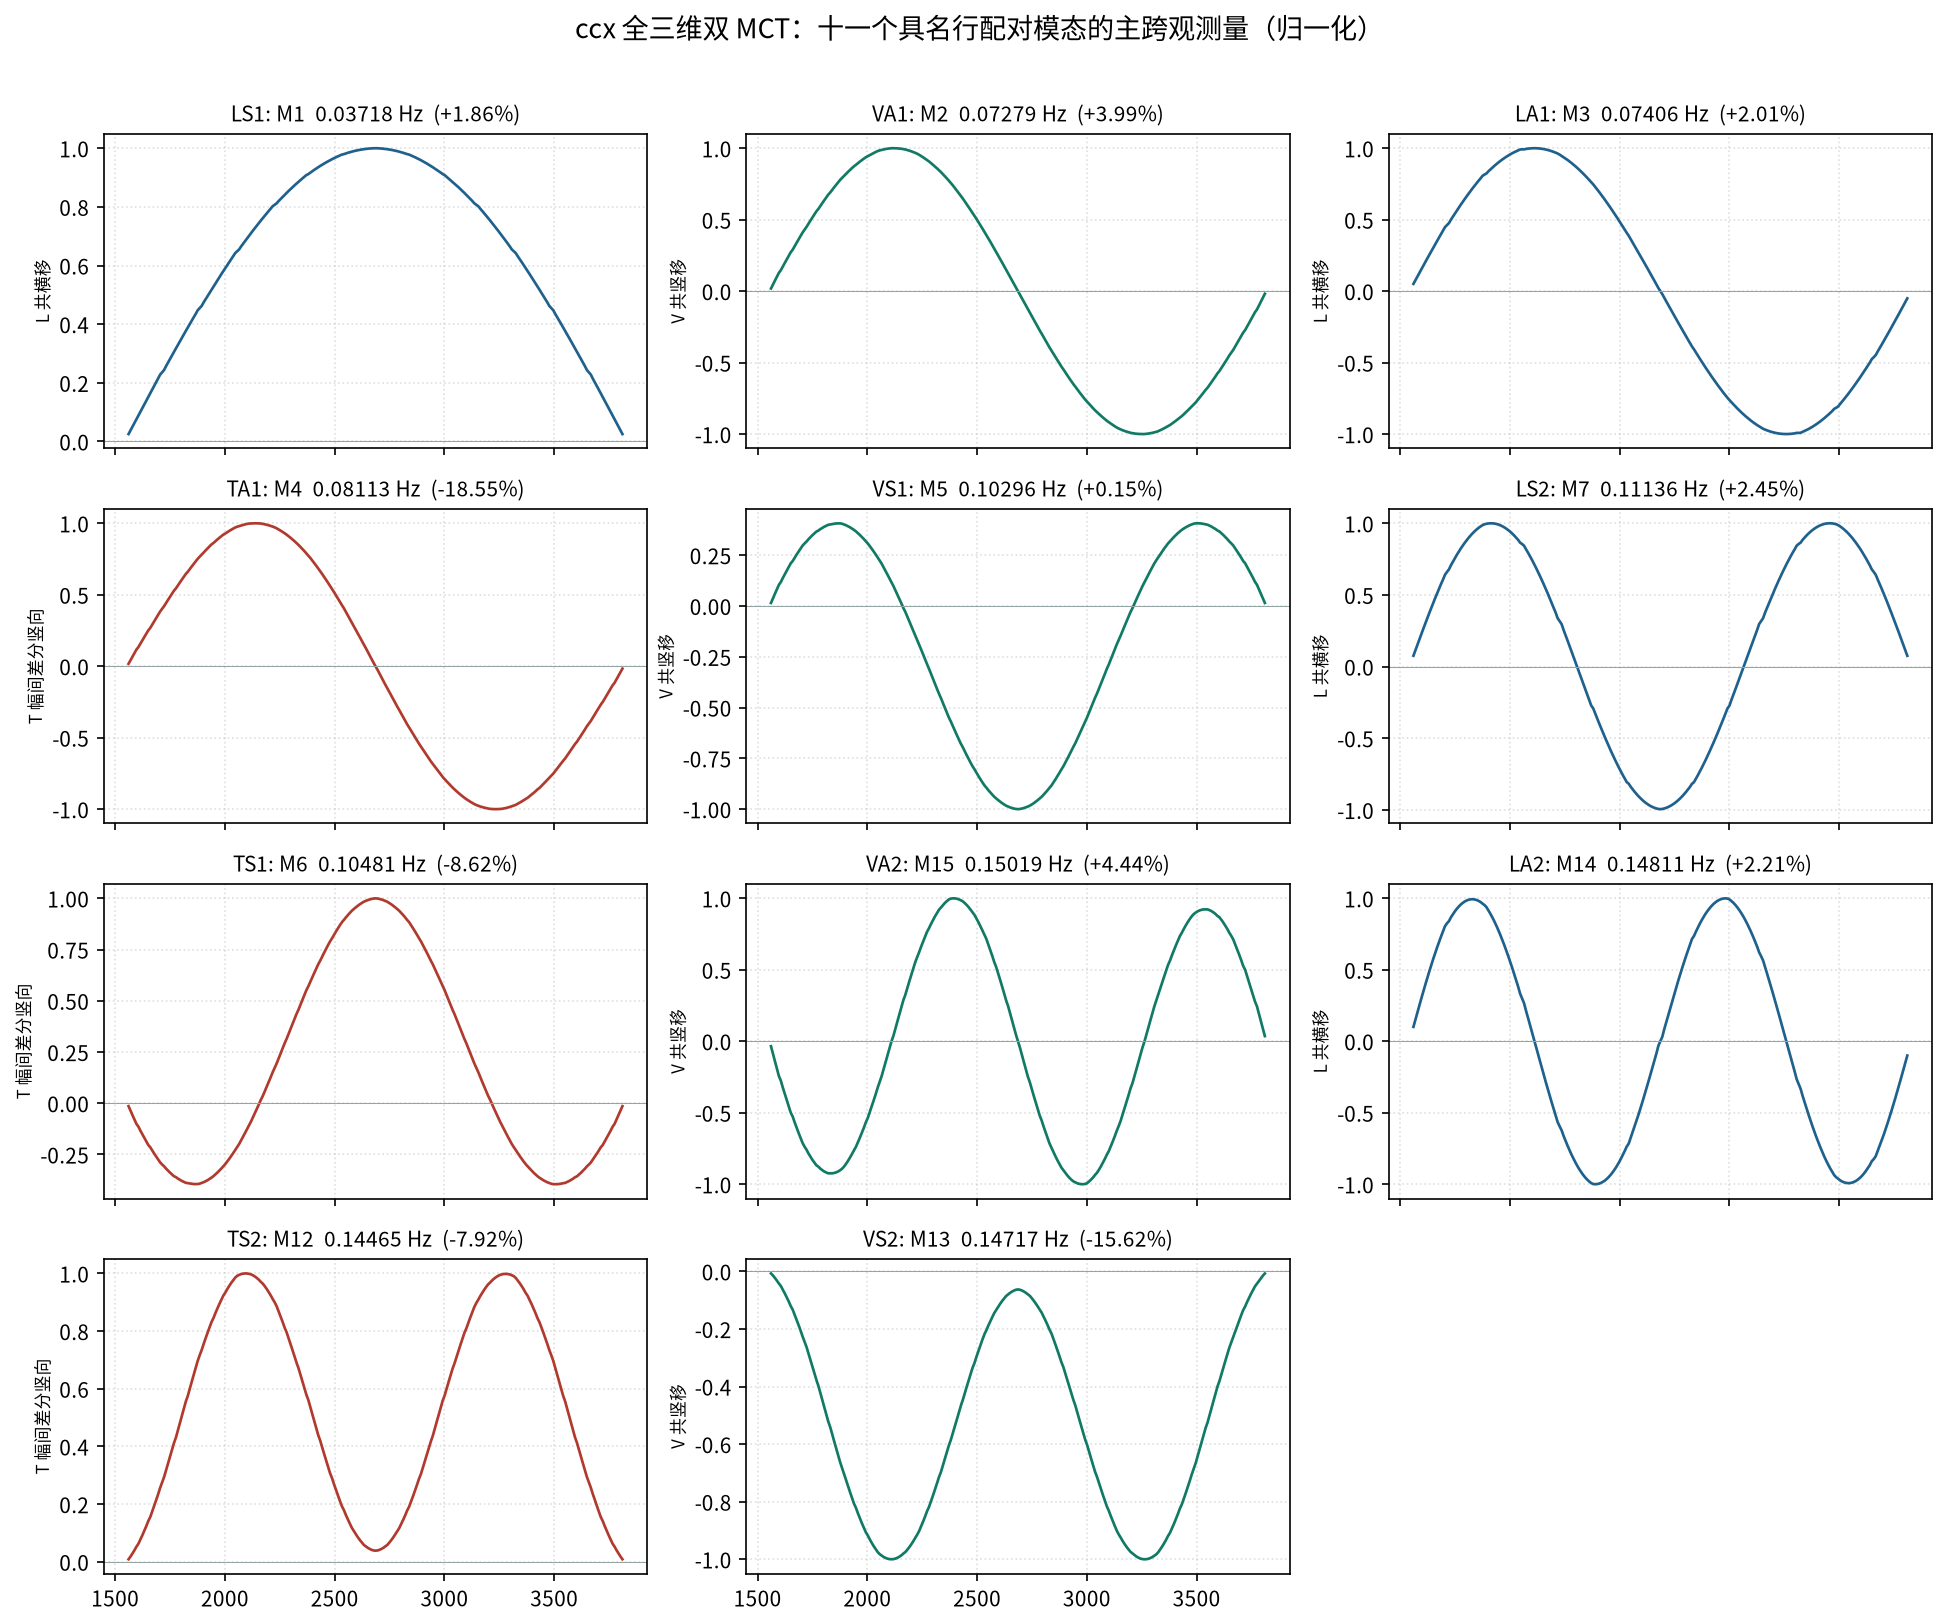
\includegraphics[width=0.99\linewidth]{../artifacts/ccx_named_mode_shapes.png}
\caption{十一个具名行的主跨观测量。TA1（M4）为幅间差分竖向双半波——与附件图 4-5 的 X 交叉同一形态。}
\end{figure}

\section{跨栈对照（S17）：括弧第三次合拢}

\begin{table}[h]\centering\small
\begin{tabular}{llrr}
\toprule
计算栈 & 连接假设 & TA1 Hz & 相对附件 \\
\midrule
ROM 图纸柔性（drawing-soft） & 滚轮/销（转动透明） & 0.07105 & $-28.66\%$ \\
ROM 滚转升级（双簇端口） & 审计凝聚（平动簇） & 0.07109 & $-28.62\%$ \\
ANSYS f99 S10--E10 & CERIG 刚臂（平动从动） & 0.07333 & $-26.38\%$ \\
\textbf{CalculiX 本次} & \textbf{共享节点焊接端（转动连续）} & \textbf{0.08113} & $\bm{-18.55\%}$ \\
ANSYS f99 E20 & COMBIN14 $k{=}10^4$（非出处） & 0.08445 & $-15.22\%$ \\
附件 2--3 & 未公开 & 0.09960 & —— \\
\bottomrule
\end{tabular}
\caption{TA1 全谱系。转动连续性是把 TA1 抬离摆式地板的真实杠杆——但图纸连接（滚轮/销）恰恰不提供转动连续；即便取焊接端上限仍差 $-18.5\%$。}
\end{table}

物理解读：焊接端把通道梁端转角锁进门架/索链，幅间差分竖向必须弯曲通道梁
（S 弯），等效每站差分竖向刚度约 2--3 N/mm，恰好给系统扭转提供了 ROM
平动端口凝聚所没有的弹性通路。这不是 ROM 的错——转角自由凝聚对应图纸的
滚轮/销连接（物理事实）；焊接端对应审计 APDL 的 CERIG 理想化（偏刚上限）。
两端夹逼下附件 TA1 仍不可达，可达域结论第三次被独立确认，且本次给出了
"上沿由什么控制"的构造性答案：\textbf{附件模型必须隐含了不低于焊接端量级的
幅间转动约束，外加其余未公开口径}。

\section{附件 2--3 其余指标汇编（S16 附录）}

按用户要求汇总附件全部可对照指标。模态与振型为本次 ccx 重算；
以下三组为 2026-08-05 审计交付包的既有结果（出处标注，本次未重跑）：

\begin{itemize}
  \item \textbf{三分力系数（附件 §3）}：西南交大 XNJD-1 风洞实测 CSV
        （$\alpha=-12^\circ\ldots+12^\circ$，$C_D$ 零攻角 $\approx0.817$ 量级曲线）
        已数字化入库并作图（\texttt{report/assets/measured\_three\_force\_coefficients.png}），
        抖振核直接采用其 PCHIP 导数。
  \item \textbf{表 5--1 抖振响应（附件 §5）}：审计频域复算（150 阶、5 种子、44.9 m/s）——
        跨中横向均值 47.86 m / $\sigma$ 18.15 m，对附件 $-72.33$ m / 19.45 m 的比值
        0.66 / 0.93（方向口径已按附件图 5-7$\sim$5-9 校正；附件缺阻尼/相干参数，
        绝对值须连同敏感性带使用）；竖向 $\sigma$ 比 0.67--1.01；
        局部扭转对照被审计明确降级（system-roll 排除后仍 1.9--45 倍，
        与 T 族可达域问题同源）。主跨单根承重索 mean$+3.5\sigma=761$ kN，
        对 2380 kN 破断比 3.13（招标验收线 $\ge3.2$，附件口径 30.1 m/s 下满足）。
  \item \textbf{表 5--2/5--3 支反力（附件 §5）}：108 个约束 DOF 独立恢复完成；
        主跨加载路径下多数锚/塔边跨反力近零，与附件全桥四跨加载不可直接互认
        （符号约定未证同一），审计包如实标注 \texttt{static\_sign\_convention\_aligned=False}。
\end{itemize}

以上与本次 ccx 静力/模态共同构成附件指标的全覆盖对照：能重算的已第三次重算，
不能客观互认的（反力符号、抖振绝对 RMS）按审计口径如实呈报而非硬配。

\section{能说 / 不能说}

\textbf{能说}：19-skill 全流程从图纸到 PDF 走通且每个 gate 有数字证据；
ccx 全三维模型质量/体积/平衡三重闭合；非 T 十一行 MAE 3.93\%；
T 族在焊接端上限下收窄到 $-18.5/-8.6/-7.9\%$，可达域括弧三栈一致；
四个 ccx 陷阱已归档为可复用的工程知识。

\textbf{不能说}：不能宣布复现表 4--1（T 族与 VS2 仍系统性偏低）；
不能把焊接端当图纸事实（图纸是滚轮/销）；不能把抖振绝对 RMS 与反力表当验收结论
（附件缺参数、符号约定未证同一）；A1--A6 是显式近似；本文 not\_a\_scientific\_claim。

\appendix
\section{复现}

\begin{verbatim}
# 生成 deck / 求解 / 后处理 / 配对 / 图件 / 工件
python3 catwalk-fem/agentic-fea/code/build_double_ccx_deck.py
cd catwalk-fem/agentic-fea/solver && ccx -i double_mct_ccx && cd -
python3 catwalk-fem/agentic-fea/code/postprocess_modes.py
python3 catwalk-fem/agentic-fea/code/pair_table41.py
python3 catwalk-fem/agentic-fea/code/plot_mode_shapes.py
python3 catwalk-fem/agentic-fea/code/emit_skill_artifacts.py
\end{verbatim}

关键哈希：MCT \texttt{0d18e3f7\ldots}；deck 见 \texttt{fem\_model\_manifest.json}；
附件 2--3 \texttt{d17d4061\ldots}；1225 图纸 \texttt{8df26c6b\ldots}。

\end{document}
